\documentclass[12pt,a4paper]{article}
\usepackage{hyperref}
\usepackage{mathtools}
\title{Template for Security-of-Wireless-Networks Reports}
\author{Vasileios Dimitrakis and Niclas Scheuing}
\begin{document}
\maketitle
\begin{figure}[h]
	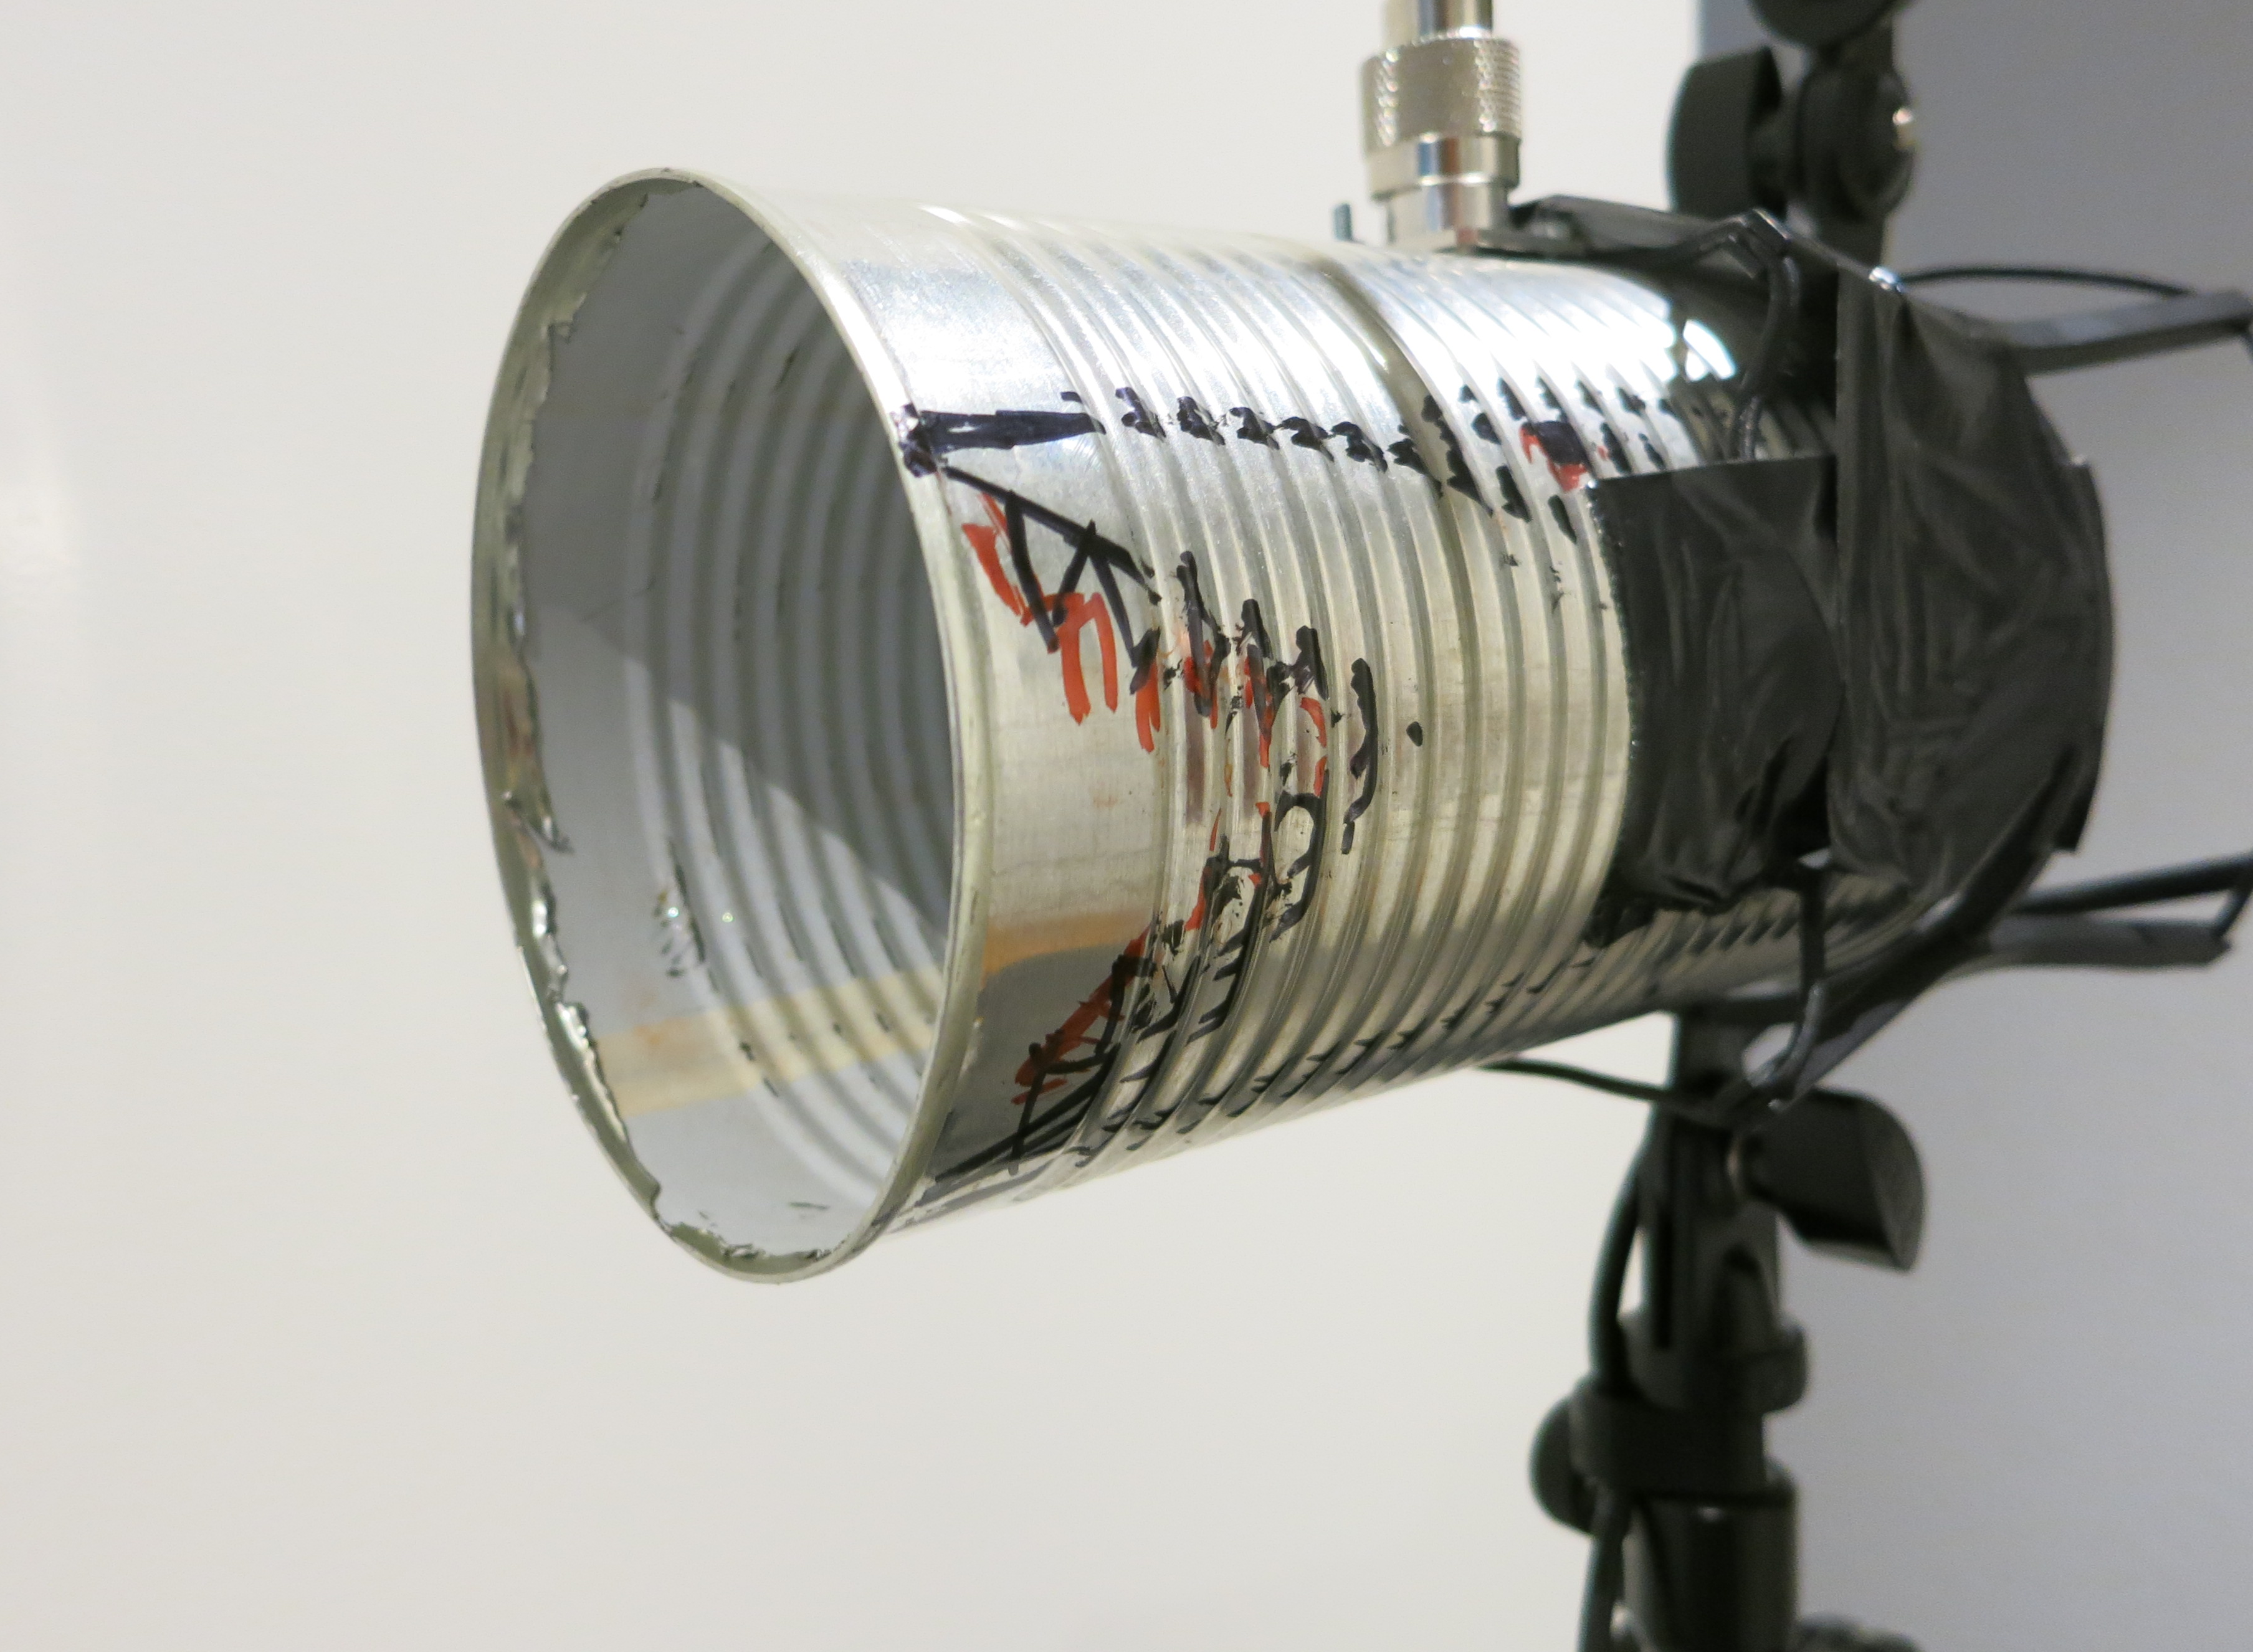
\includegraphics[width=\textwidth]{images/shark_cut.png}
	\caption{Cantenna}
	\label{shark}
\end{figure}
\pagebreak
\section{Introduction}
The objective of this exercise is the creation and the performance evaluation of a high gain
and directional Wi-Fi antenna. The effectiveness of the antenna will be evaluated in comparison with an omnidirectional and a professional Wi-Fi antenna. The design that we chose to build is a cantenna. Cantenna is a homemade directional waveguide antenna, made out of an open-ended metal can.
\subsection{Materials}
The materials and the equipment that were used for the creation and the setup of the antenna are the following: 
\begin{itemize}
\item {\emph{$1$ USB Alfa wireless adapter:} Is the client associated with the Access Point.} 
\item {\emph{$1$ TP-Link wireless adapter:} Is used as the Access Point.}
\item {\emph{$1$ Pigtail cable:} Is used to connect the cantenna with the USB Alfa wireless adapter.}
\item {\emph{$1$ female N-connector}}
\item {\emph{$1$ piece of copper wire:} Is used as the active element, the monopole, that radiates the waves}
\item {\emph{$1$ cylindrical can:} Plays the role of the Wi-fi antenna.} 
\end{itemize}
The cantenna used in this exercise will use the Wi-Fi channel $6$ with central frequency $2.437$GHz and wavelength $12.31$cm.

\section{Theoretical background of the cantenna}
The cantenna, as it was described in the introduction, is a directional waveguide antenna and in our case, it is also a cylindrical cantenna. This kind of waveguide supports both traverse electric (TE) and traverse magnetic (TM) modes. The traverse modes are a particular electromagnetic field pattern of radiation measured in a plane perpendicular (i.e., transverse) to the propagation direction of the beam. They have a cutoff frequency, below which electromagnetic energy is severely attenuated and above this, the certain mode is excited. An ideal cantenna has only one mode, the dominant one, which is the TE\textsubscript{11}, because our cantenna is a cylindrical waveguide. If the cantenna excites more than one modes, this phenomenon will decrease the effectiveness of the antenna, because the energy of the electromagnetic wave will be spread within different modes. The mode that we do not want to trigger is the TM\textsubscript{10}. In the following, Figure 1 presents a cantenna setup.



\subsection{Cantenna design parameters}
\subsubsection{Can diameter}
As we described in the introductory part of the cantenna theory, the cantenna has to trigger only the dominant mode TE\textsubscript{11}, which has the lowest cutoff frequency. For frequencies lower than the previous one, no mode is triggered, because waves are attenuated exponentially. The second mode is the TM\textsubscript{10} and if the frequency is greater than the one of TM\textsubscript{10}, both the two first modes will be excited. Considering all the above, we deduce that the Wi-Fi frequency f\textsubscript{Wi-Fi} has to fulfill the following inequality:
\begin{equation}
	f_{TE_{11}} < f_{Wi-Fi} < f_{TM_{10}}
\end{equation}
.
According to the citation\cite{waveguide}, the formulas for the above two frequencies for the cylindrical waveguide are the following:
\begin{equation}
	\frac{p_{11} c}{\pi f_{WiFi}} < D < \frac{p_{01}' c}{\pi f_{WiFi}}
\end{equation}
%TODO: are the p values correct?
where $p_{11} = 1.841$ and $p_{01}'= 3.832$ are parameters related to the Bessel function, $c$ the speed of light.
%TODO: also provide the final values for the equation above
Therefore, according to these theoretical values, the diameter of our cantenna has to be between these limits. Although these are the theoretical values of the diameter, in real cases, it has to be approximately between 8-11cm, so that the antenna will be effective.

\subsubsection{Position of the copper element: Acts as the monopole}

The electromagnetic wave of the Wi-Fi signal is transmitted through the air and reaches the opening of our cantenna. Inside the can and according to the frequency of the wave, one or more modes are excited. Moreover, the wave inside the can is reflected to the bottom and this results in the creation of a static wave. The wavelength $\lambda_g$ of the wave in the internal of the can is equal to the wavelength of the mode that is triggered. In our case we want to trigger only the dominant mode f\textsubscript{TE\textsubscript{11}}. Moreover, we have to take into consideration the creation of the static wave and decide which is the best position of the monopole, so that the effectiveness of our antenna will be the highest. It is known from the wave theory, that the peak of a static wave is presented in distance $\frac{\lambda_g}{4}$ from the can bottom. Taking into consideration this wave property, we opened a hole on the can $4.1$cm from the can bottom. 

\subsubsection{Monopole length}
As we described in subsection 2.1.2, the monopole is placed $\frac{1}{2}\times{λ\textsubscript{g}}$ from the bottom of the can and its orientation is vertical to the internal side of the can. The monopole antenna is a class of radio antenna consisting of a straight rod-shaped conductor, often mounted perpendicularly over some type of conductive surface, called a plane ground. In our case, we decided to built the most common type of the monopole, which is the quarter-wave monopole. It is also called Marconi antenna from the name of its inventor. This monopole is ideal for our configuration, because it is simple and it has the right dimensions, in order to fit inside the cantenna. The length of the monopole, as we said before, is equal to $\frac{1}{4}\times{λ\textsubscript{Wi-Fi}}$. The λ\textsubscript{Wi-Fi} is the wavelength of the signal transmitted in the free space. In the current setup, the wavelength is equal to 12.3cm, so the length of the monopole is approximately 3.1cm.

\subsubsection{Length of the can}
The length of the can has to be more than $\frac{3}{4}\times{λ\textsubscript{g}}$. The longer the cantenna is the more directional and effective becomes. In our case, the length of the cantenna is $16$cm, so we expect to be directional and effective.

\subsection{Cantenna theoretical and experimental device dimensions} 
In Table 1, we present the theoretical design parameters of the cantenna and the actual ones of our setup. It is clear from the table that our cantenna satisfies all the design prerequisites and thus, we expect to receive very good results, as far as the antenna gain and the directivity are concerned.

\begin{table}
	\begin{center}
		\begin{tabular}{r|r|r|r}\
		 & Theoretical value in mm& Actual Values in mm\\
		 \hline 
		 \emph{Can diameter} & 0 & 100.5\\
		 \emph{Monopole position} & 0 & 44.1 \\
		 \emph{Monopole length} & 0 & 30.75\\
		 \emph{Length of the can} & 0 & 162.5\\
		\end{tabular}
	\end{center}
\end{table}

\section{Setup}
	\begin{figure}
		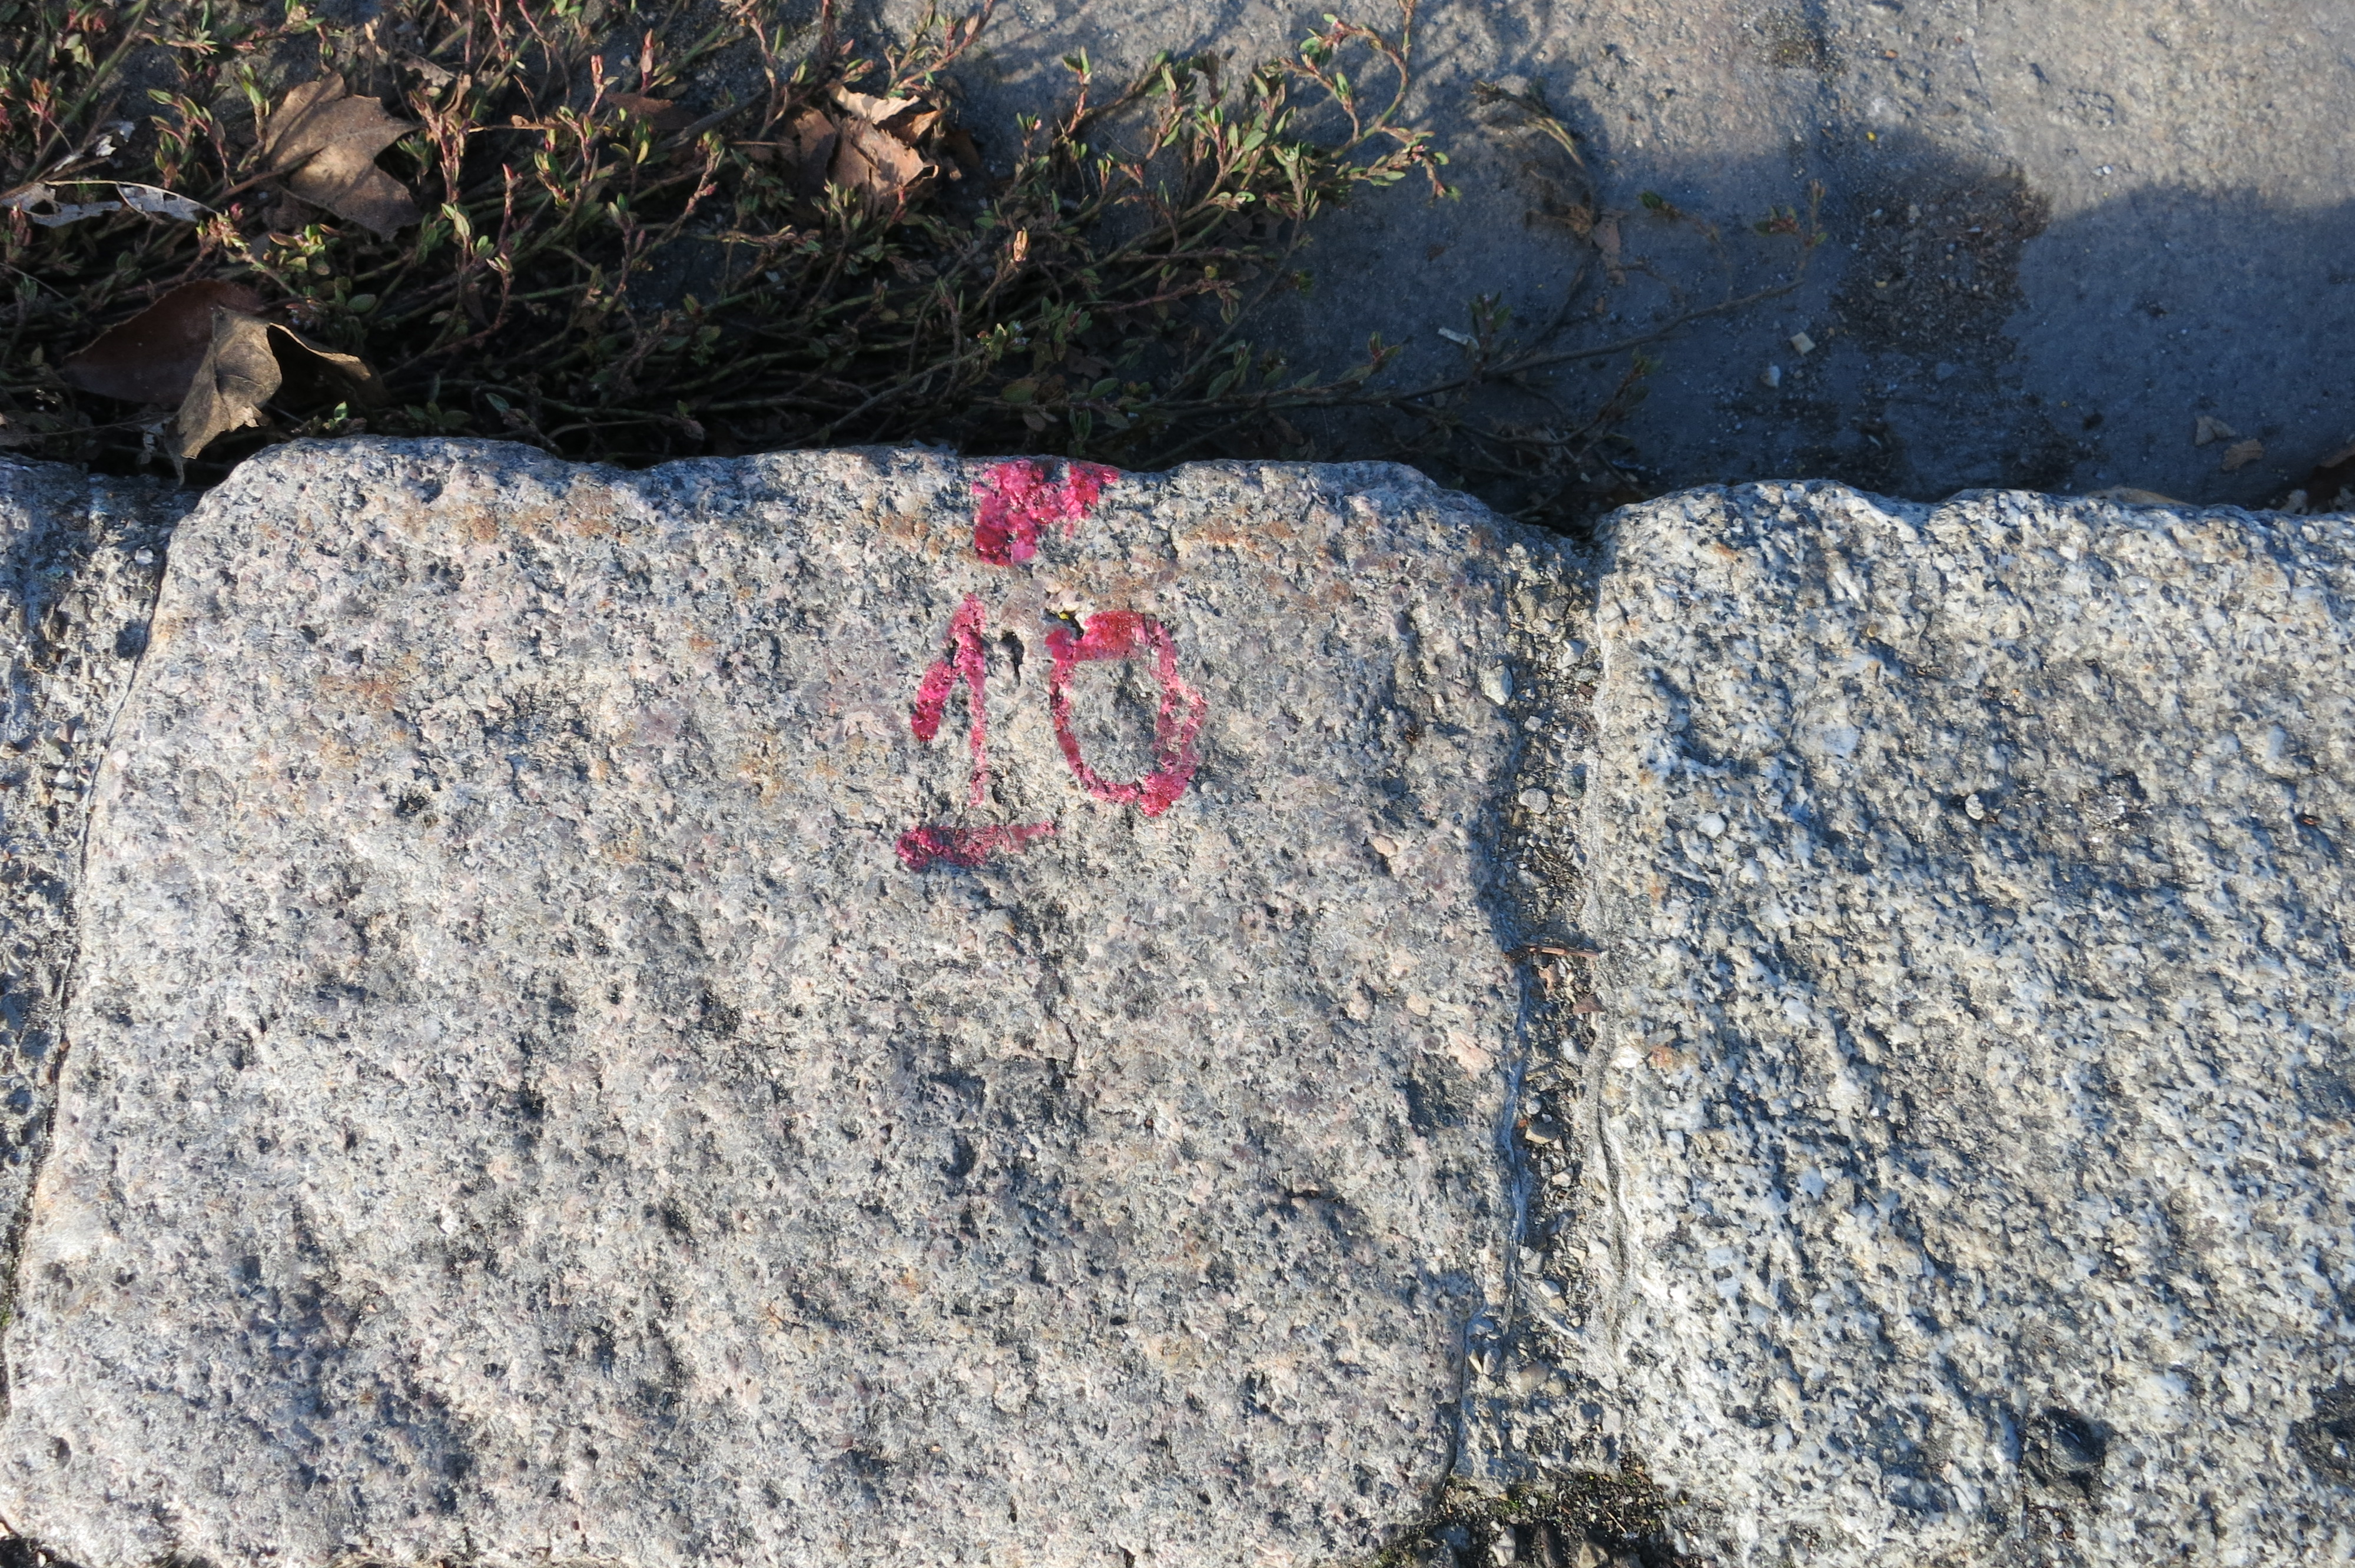
\includegraphics[width=\textwidth]{images/marks.JPG}
		\caption{title}
		\label{marks}
	\end{figure}
	\begin{figure}
		\includegraphics[angle=270,width=\textwidth]{images/setup.JPG}
		\caption{title}
		\label{setup}
	\end{figure}

\section{Results}
This section is divided in two different subsections: The one is the Gain measurements and the other is the Directionality measurements. 

\subsection{Gain measurements}
In this phase of our experiment, we will compare the way that the signal strength changes increasing the distance of the AP and the antenna under test (client). This experiment will be executed for three different antennas: an omnidirectional antenna, a professional cantenna and our cantenna. In order to be the measurements accurate, they have to be taken in an open area field. For this reason, we chose the place, that is depicted in the following pictures, in order to avoid environmental effects, such as reflections by buildings, scattering by moving objects.

\subsection{Directionality measurements}
The second phase of the experiment evaluates the directionality of each of the above antennas. All the measurements for the three antennas will be taken in $20$m distance from the Access Point. The starting point of the measurements will be considered the one with $0degrees$. Every next measurement will be taken every 20degrees.

\subsection{Maximum distance measurements}
\begin{figure}
	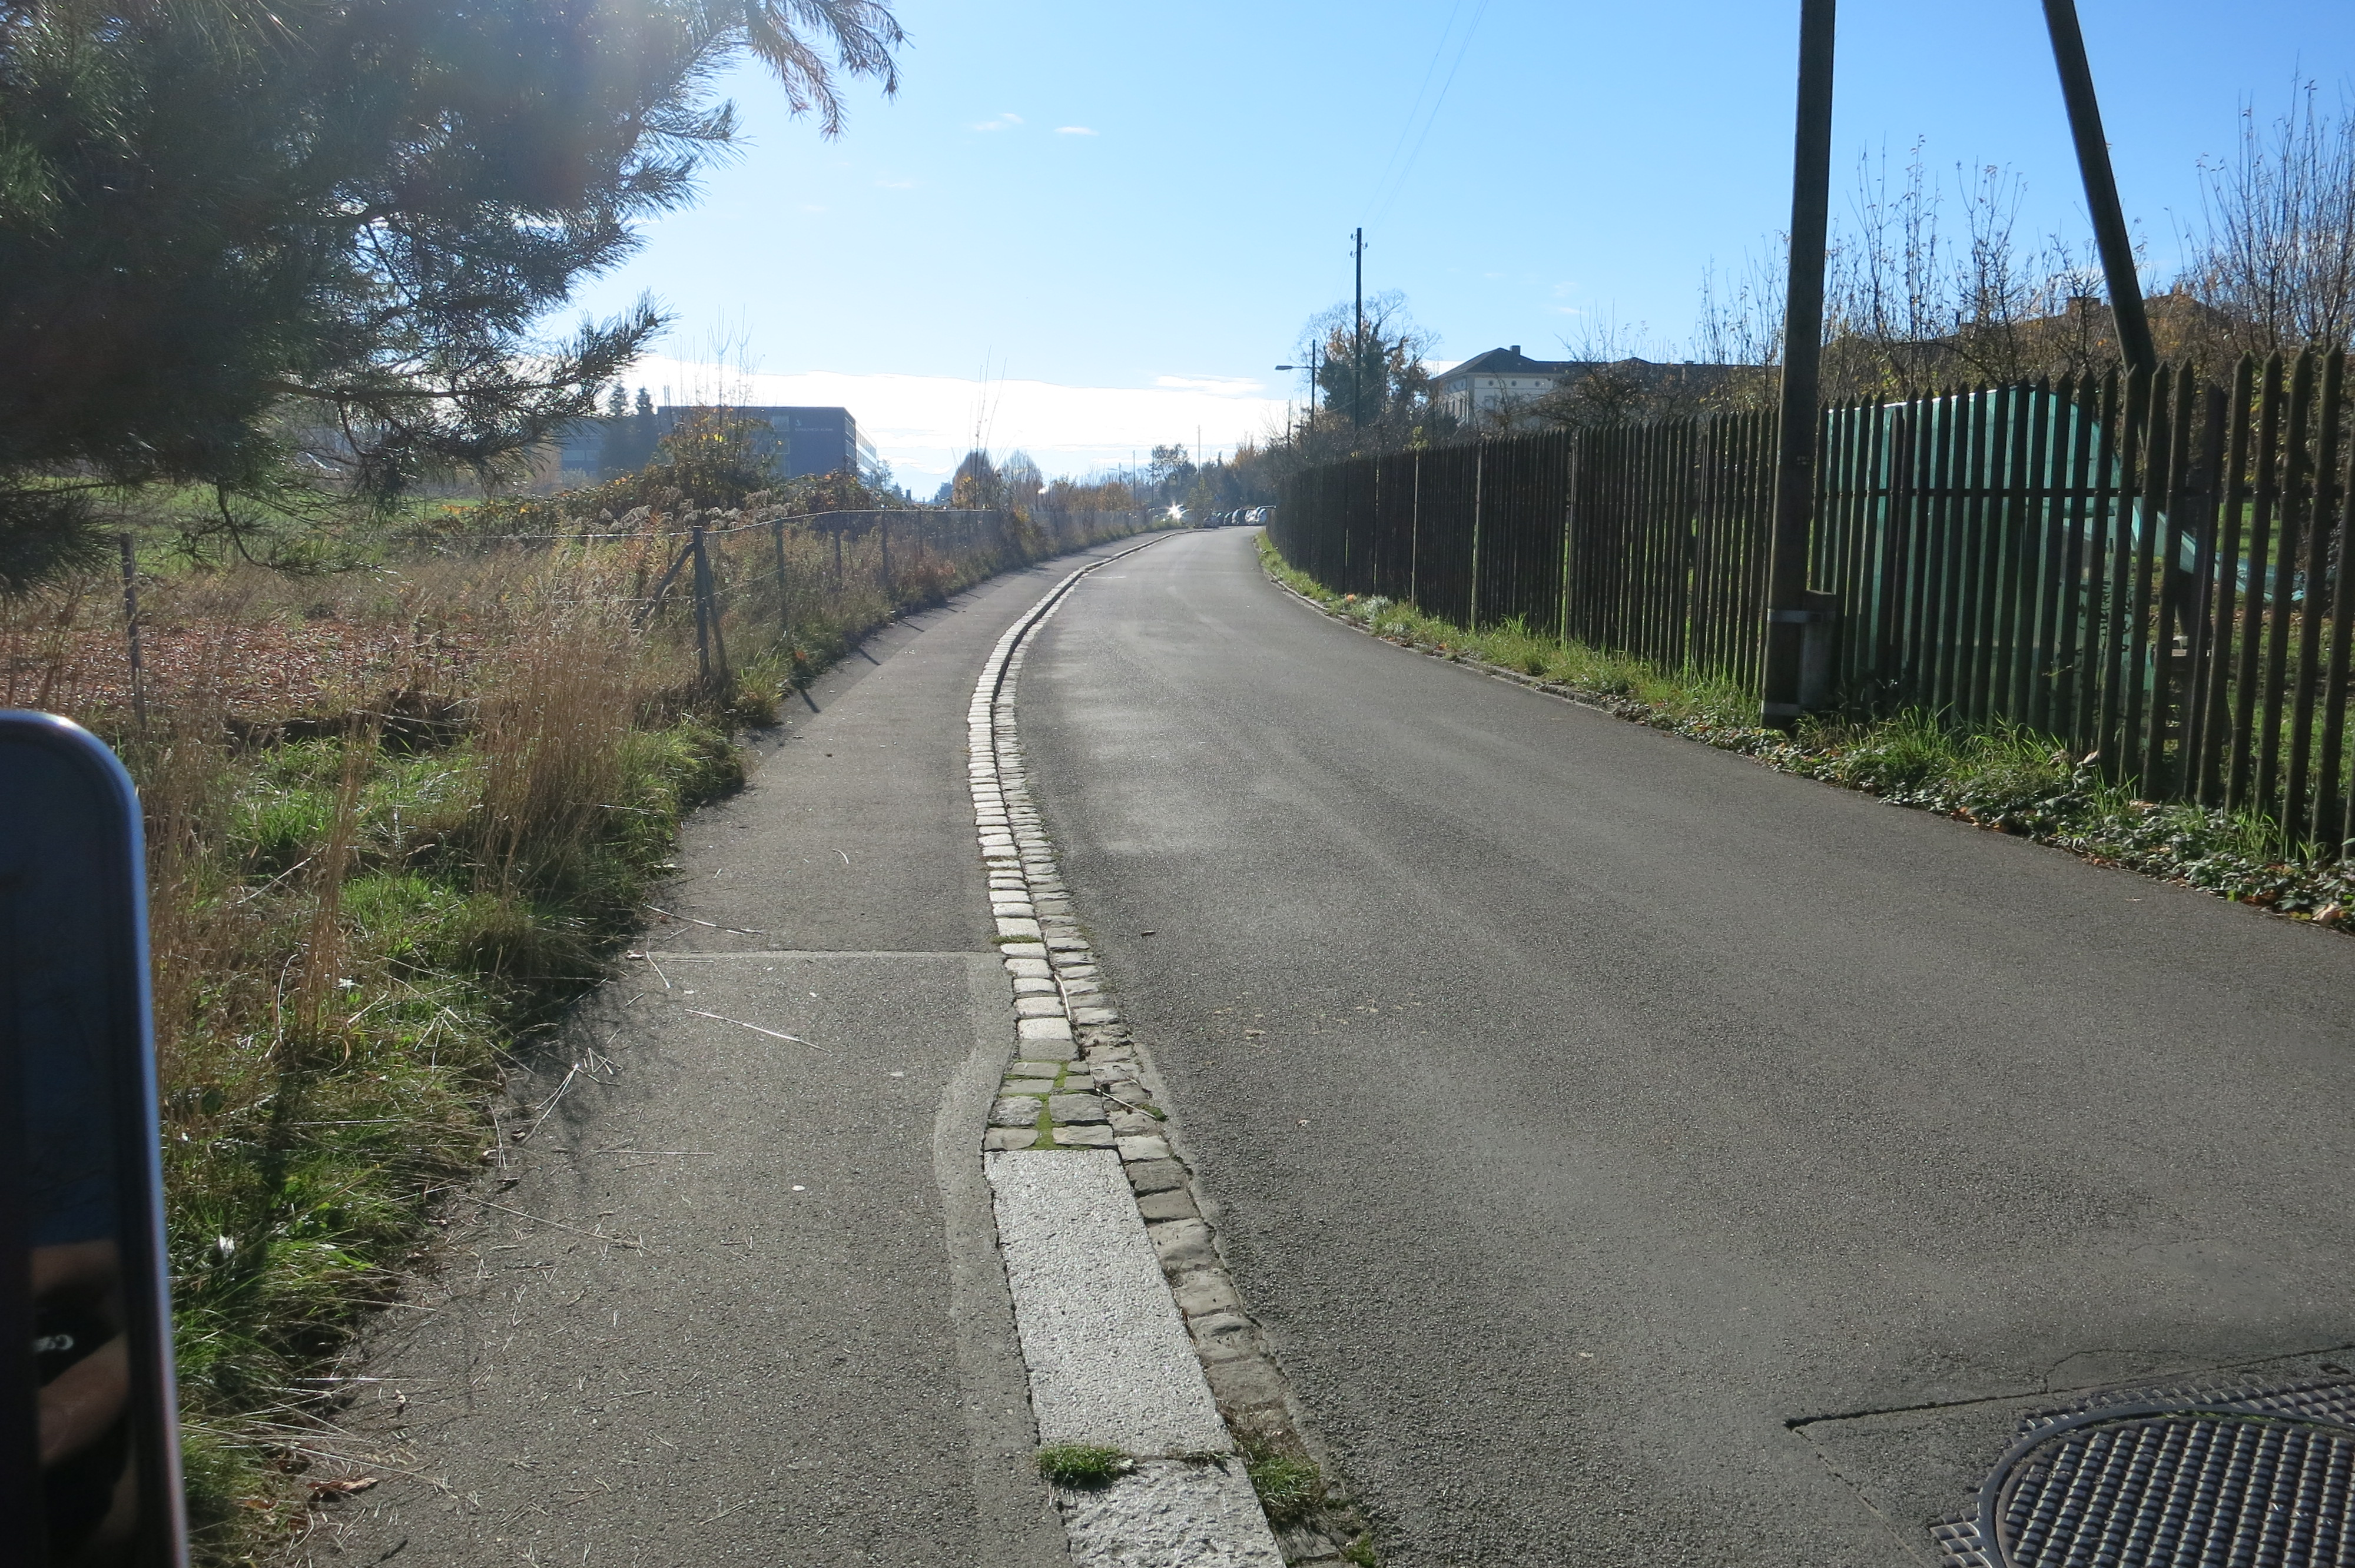
\includegraphics[width=\textwidth]{images/distance.JPG}
	\caption{title}
	\label{distance}
\end{figure}

\begin{figure}
	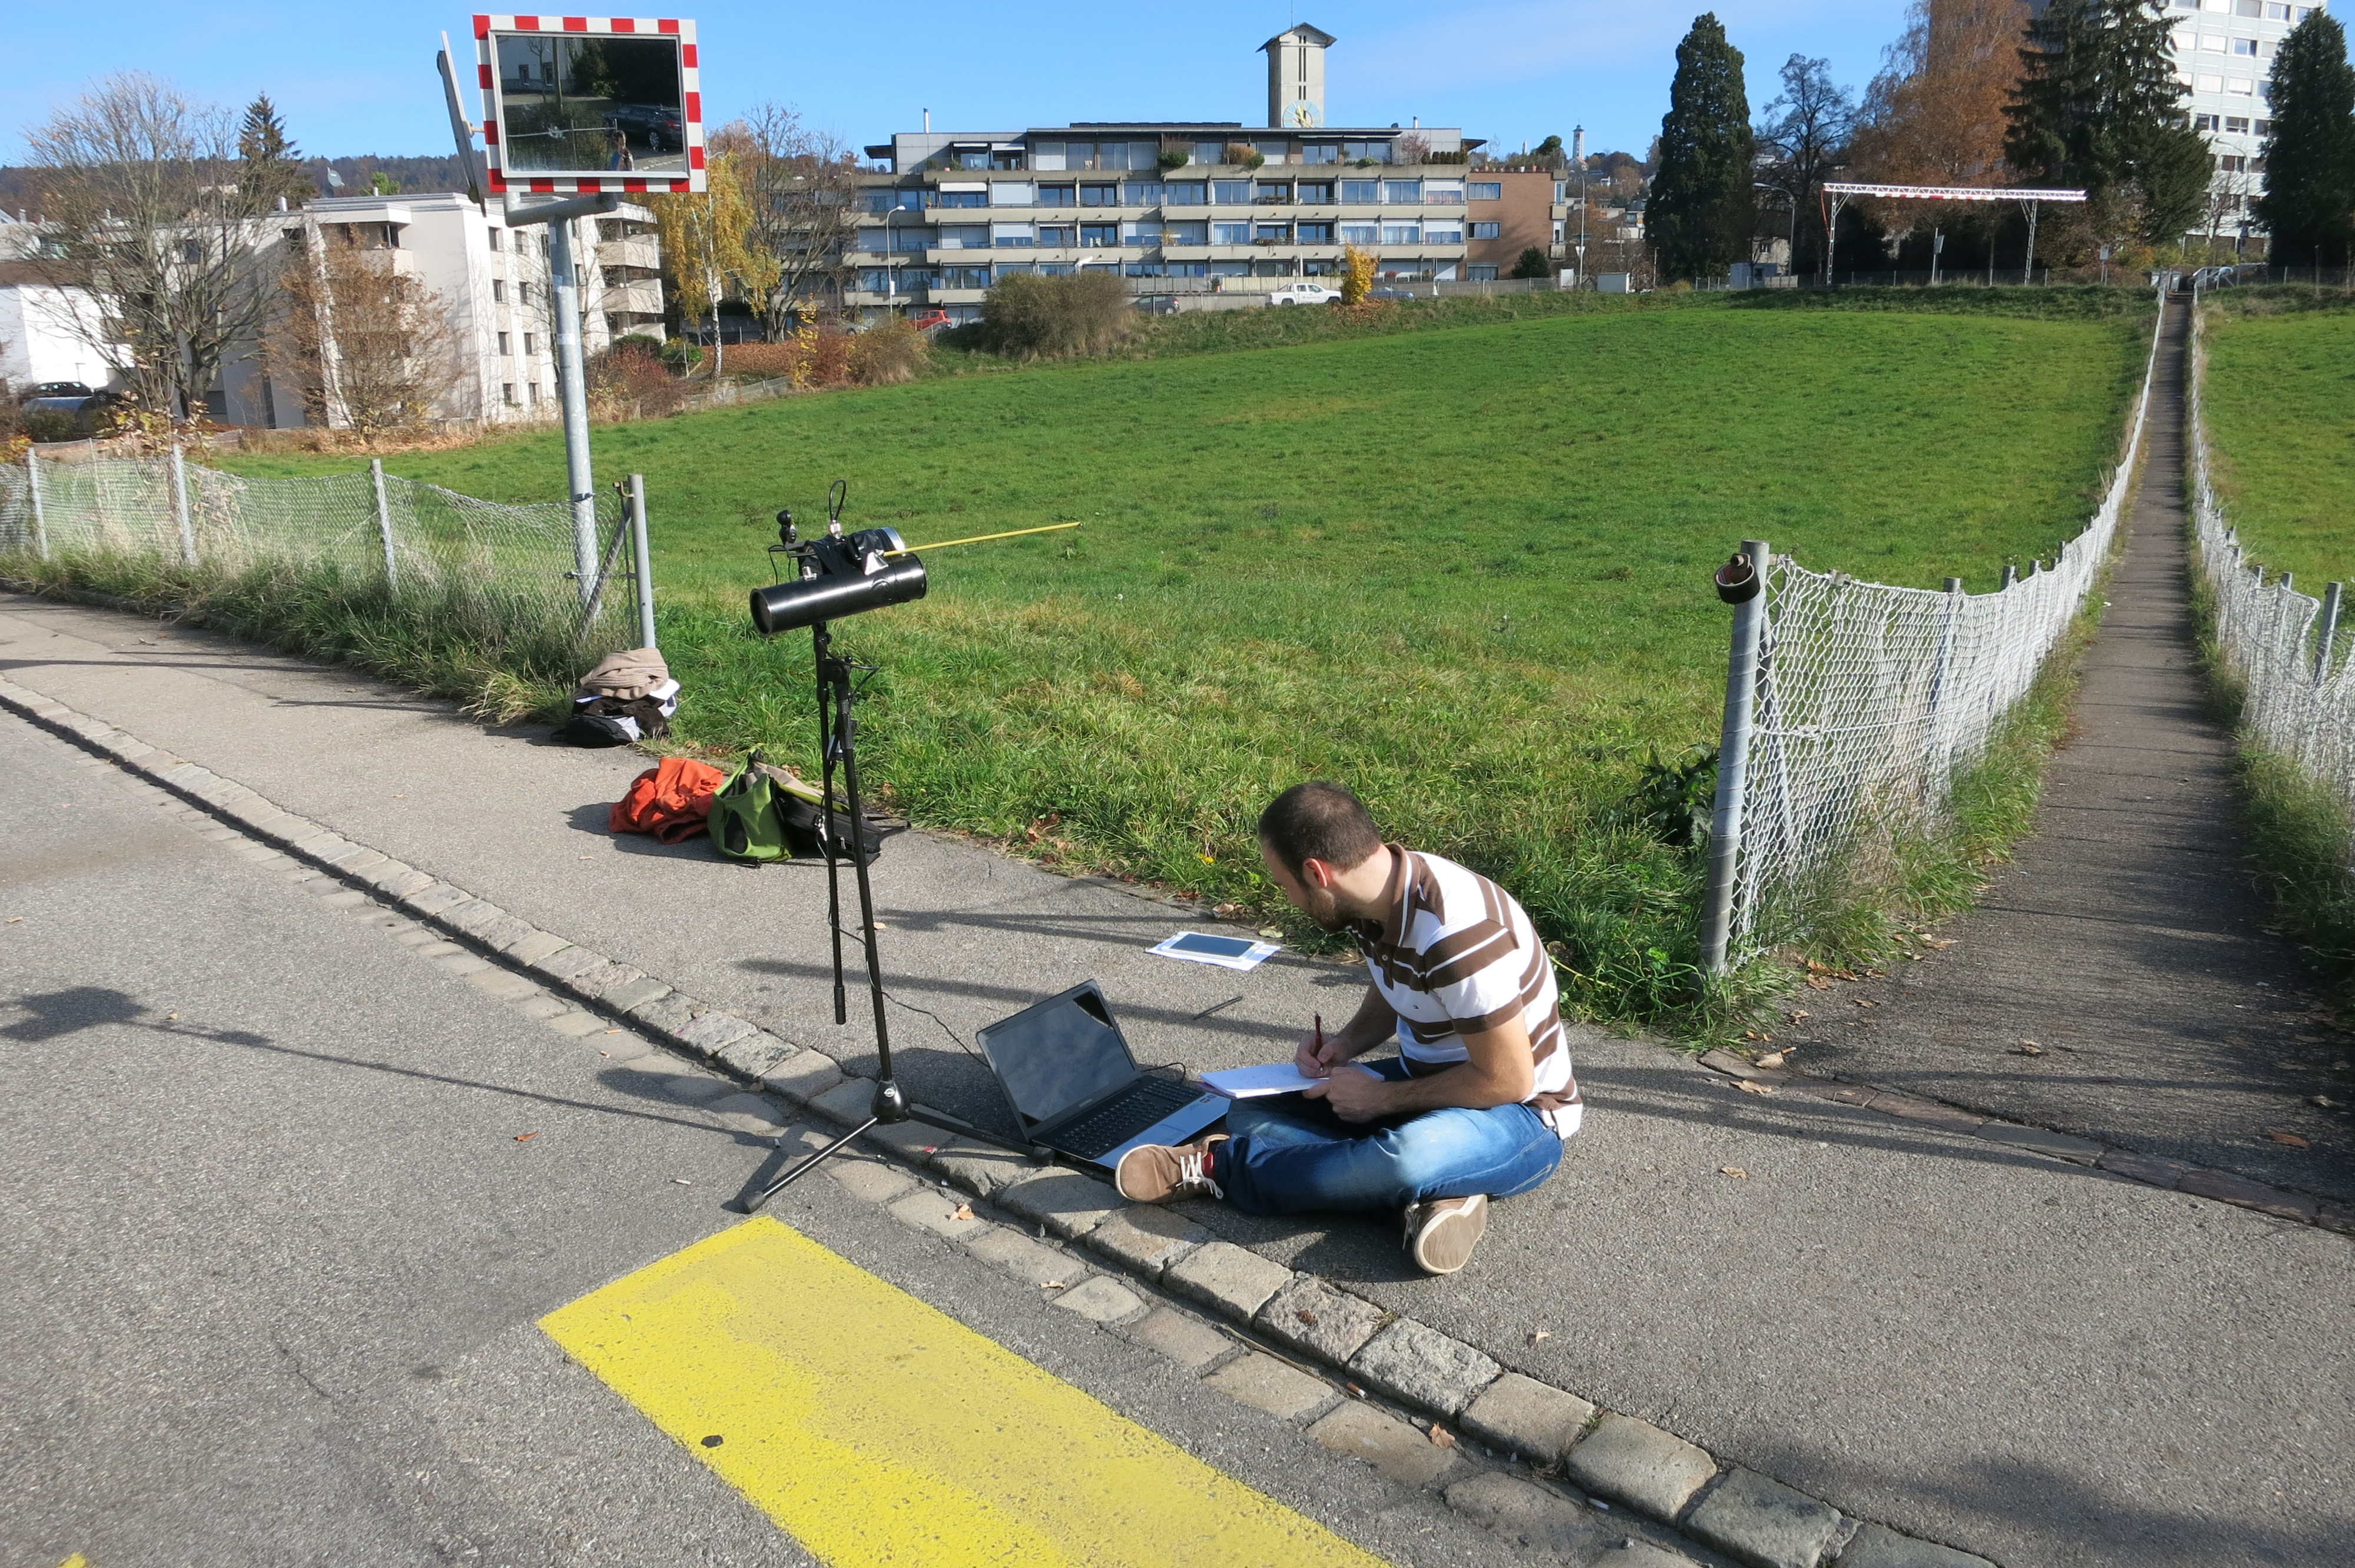
\includegraphics[width=\textwidth]{images/cool.JPG}
	\caption{title}
	\label{cool}
\end{figure}




\section{Analysis}
\bibliographystyle{plain}
\bibliography{bibliography}
\section{Appendix}
%cantenna

\begin{table}
	\begin{center}
		\begin{tabular}{r|r|r}\
		 Distance in $m$ & signal strength in $dBm$ & transfer rate in $Kib/s$\\
		 \hline 
		 1 & -4 & 520\\
		 10 & -16 & 5649\\
		 20 & -25 & 5024\\
		 40 & -27 & 5194\\
		 60 & -32 & 6386\\
		 80 & -37 & 5933\\
		 100 & -42 & 6300\\
		\end{tabular}
	\end{center}
	\caption{Our cantenna. Measured signal strength and bandwidth depending on the distance}
	\label{dist:can}
\end{table}

%prof cantenna
\begin{table}
	\begin{center}
		\begin{tabular}{r|r|r}\
			Distance in $m$ & signal strength in $dBm$ & transfer rate in $Kib/s$\\
			\hline 
			1 & -4 & 389\\
			10 & -20 & 8500\\
			20 & -33 & 8400\\
			40 & -28 & 9300\\
			60 & -30 & 8200\\
			80 & -36 & 7900\\
			100 & -40 & 7800\\
		\end{tabular}
	\end{center}
	\caption{Professional cantenna. Measured signal strength and bandwidth depending on the distance}
	\label{dist:prof}
\end{table}

%onmi cantenna
\begin{table}
	\begin{center}
		\begin{tabular}{r|r|r}\
			Distance in $m$ & signal strength in $dBm$ & transfer rate in $Kib/s$\\
			\hline 
			1 & -4 & 2700\\
			10 & -22 & 6400\\
			20 & -24 & 5900\\
			40 & -27 & 6100\\
			60 & -25 & 5600\\
			80 & -37 & 5800\\
			100 & -39 & 5200\\
		\end{tabular}
	\end{center}
	\caption{Omni-directional antenna. Measured signal strength and bandwidth depending on the distance}
	\label{dist:omnio}
\end{table}


% cantenna angular
\begin{table}
	\begin{center}
		\begin{tabular}{r|r|r}\
			Angle in degrees $m$ & signal strength in $dBm$ & transfer rate in $Kib/s$\\
			\hline 
			0 & -30 & 6600\\
			20 & -32 & 5200\\
			40 & -36 & 5400\\
			60 & -40 & 5700\\
			80 & -46 & 6000\\
			100 & -54 & 6800\\
			120 & -52 & 8000\\
			140 & -52 & 9600\\
			160 & -54 & 8200\\
			180 & -52 & 9500\\
			200 & -52 & 9600\\
			220 & -53 & 9900\\
			240 & -54 & 10100\\
			260 & -49 & 9900\\
			280 & -47 & 10100\\
			300 & -39 & 9800\\
			320 & -33 & 7300\\
			340 & -32 & 6800\\
		\end{tabular}
	\end{center}
	\caption{Our cantenna. Measured signal strength and bandwidth depending on the angle}
	\label{ang:can}
\end{table}

% prof cantenna angular
\begin{table}
	\begin{center}
		\begin{tabular}{r|r|r}\
			Angle in degrees $m$ & signal strength in $dBm$ & transfer rate in $Kib/s$\\
			\hline 
			0 & -37 & 7900\\
			20 & -39 & 7100\\
			40 & -42 & 7200\\
			60 & -43 & 7300\\
			80 & -48 & 8200\\
			100 & -52 & 9300\\
			120 & -51 & 9900\\
			140 & -53 & 9600\\
			160 & -55 & 9400\\
			180 & -48 & 10300\\
			200 & -51 & 10300\\
			220 & -55 & 9200\\
			240 & -53 & 9800\\
			260 & -48 & 10300\\
			280 & -42 & 10300\\
			300 & -39 & 10300\\
			320 & -37 & 7900\\
			340 & -36 & 7700\\
		\end{tabular}
	\end{center}
	\caption{Pofessional cantenna. Measured signal strength and bandwidth depending on the angle}
	\label{ang:prof}
\end{table}

% omni angular
\begin{table}
	\begin{center}
		\begin{tabular}{r|r|r}\
			Angle in degrees $m$ & signal strength in $dBm$ & transfer rate in $Kib/s$\\
			\hline 
			0 & -36 & 6400\\
			20 & -42 & 6300\\
			40 & -44 & 6100\\
			60 & -44 & 6200\\
			80 & -43 & 7300\\
			100 & -42 & 7300\\
			120 & -38 & 7600\\
			140 & -40 & 7400\\
			160 & -42 & 7400\\
			180 & -46 & 7100\\
			200 & -37 & 7300\\
			220 & -39 & 6700\\
			240 & -42 & 7300\\
			260 & -42 & 6500\\
			280 & -42 & 6900\\
			300 & -42 & 5900\\
			320 & -41 & 2400\\
			340 & -42 & 3100\\
		\end{tabular}
	\end{center}
	\caption{Omni-directional antenna. Measured signal strength and bandwidth depending on the angle}
	\label{ang:omni}
\end{table}
\end{document}